\chapter{Related Work: Creative Problem-Solving}

Take the problem $2 + 2$. The solution to this problem is true in all cases. There may be a few different ways to solve the problem, such as counting on one’s fingers or creating two separate groups of two apples and counting, but the answer is the same and remains the only definitive answer. Now take a problem like decorating a living room. There are principles such as color theory and strategies that designers use, but the outcome of the room itself can vary vastly, and there is not single correct answer to what the room should look like. This is what differentiates creative thinking from other types of problem-solving: creative thinking is one in which both the goal and the solution are open-ended. In problem-solving --creative or otherwise-- we engage solution-generating processes of finding all potential paths and verifying processes of choosing among those paths to find a ``solution’’ \cite{Newell1962processes}. The solution-generation process is the ``hot'' exploratory phase of searching a wide and diverse semantic space and uncovering a breadth of possible ideas; the verifying process then ``cools'' to exploit, searching a narrower semantic space to refine among potential solutions \cite{kirkpatrick1983optimization, lucas2014children}. The process of exploration (the how) focuses on ideation and thinking about a breadth of alternatives; the content of exploration (the what) focuses on application of ideas and accomplishing goals \cite{Kelley2013, kemp2007learning, Newell1962processes, osborn1953applied}. Exploration for structured problems where a single optimal solution exists and can be assessed through objective measures of correctness (\textit{e.g.} solving an arithmetic problem, checking for spelling errors) is straightforward. However, creative, open-ended problems do not have a single or ``correct’’ solution and are assessed based on contextual means other than distinct correctness, making both process and content exploration inherently ambiguous. 


\section{Getting ``Unstuck'': From a Fixation Bias to Action}
People use analogical thinking to handle and manage ambiguity, drawing upon both superficially and structurally similar representations and ideas for problem-solving \cite{gentner1983structure, Gentner2010, gick1980analogical, tversky1973availability, vanlehn1998analogy}. A classical example of this is applying the analogy of assembling an army for battle to treating cancer \cite{duncker1945problem, gick1980analogical}. Analogical thinking forms the basis of creativity, making conceptual leaps through connecting semantically distant, yet relational analogies \cite{chan2011benefits, gentner1997analogy, gentner2003learning, Green2016, vendetti2014far}. People are often drawn to concrete,  superficial features because they are more salient. However, focusing too much on the low-level superficial features hinders the ability to see the underlying structure and make further conceptual leaps  \cite{gentner1983structure, gick1980analogical, lucas2014children, vendetti2014far}. For example, in the classical example of applying the analogy of assembling an army for battle, people were less likely to notice the far analogy without a hint because the two scenarios seemed too different, at least on the surface \cite{gick1980analogical}. 

People often have a cognitive bias to settle too quickly on a single approach when they might be better served by exploring more broadly \cite{jansson1991design, kershaw2004, Ohlsson1992, simon1972theories}. Novices especially often lose sight of the forest for the trees, getting mired in details and finding it difficult to take a step back. One reason may be a tendency to engage in fast or automatic thinking rather than effortful thinking to see past details \cite{allen2011dual, kahneman2011thinking}. A person might wonder why they should ``waste time’’ on a path that they do not ultimately pursue. Another reason is an availability bias where the information readily available is the only possible range of outcomes \cite{tversky1973availability}. Lack of expertise is a potential third reason. Unlike novices who get bogged down by the trees, experts are often able to see the abstract forest, recognizing patterns and creating structural units of these patterns through `chunking’ \cite{Chase1973, chi1981categorization, ericsson2018cambridge, Gobet2001,Gobet1998}. When asked to categorize various physics problems, novices categorized them based on superficial features such as whether the problems included a plane or ramp while experts categorized these problems based on their concept such as whether the problem could be solved by the work-energy theorem \cite{chi2012seeing,chi1981categorization}. Yet expertise is not the panacea for catalyzing exploration. Inflexible, rote expertise might instead be more of an anchor to new and more flexible ways of thinking \cite{hinds1999curse, hinds2001, wiley1998expertise}. 

Hatano differentiates routine expertise from a more situational form of expertise known as \textit{adaptive expertise} \cite{Hatano}. Adaptive expertise emphasizes transfer of knowledge to new contexts and problems, knowing how and when to apply knowledge through different strategies \cite{Schunn2005}. In the face of ambiguity as in creative problem-solving, adaptive expertise and analogical thinking function in parallel, prospectively mapping known representations to new and seemingly distant situations \cite{chan2011benefits, gentner1997analogy, Green2016, schwartz2005efficiency, Smith1993}. For example, in a study where graduate students and undergraduate students performed a medical diagnosis task, graduate students proactively made external representations that allowed them to perform better at task despite both groups being novices in the medical domain \cite{Lee2009}. Expertise alone does not explain the ability to explore, but rather it may be the strategies and the contexts in which expertise is applied that enable greater creativity. In learning situational knowledge and building adaptive expertise, the challenge is orienting people towards an epistemological middle ground of how to find the right design and how to get the design right \cite{Buxton2007, tohidi2006getting}. The remainder of this chapter will discuss strategies and tools for helping people move away from fixation towards action and exploration.

\begin{figure}[b!]
\centering
  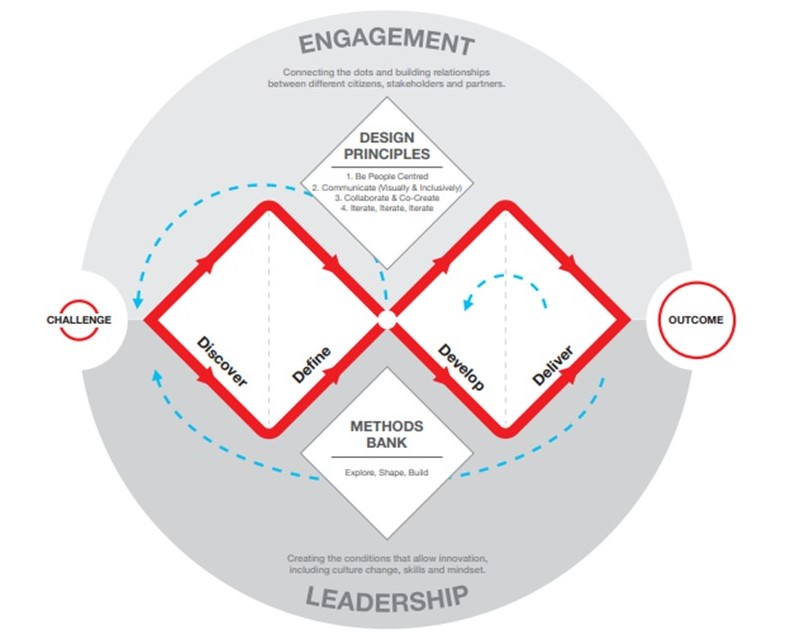
\includegraphics[width=.7\textwidth]{i_figures/double_diamond.jpg}
  \caption{The British Design Council created this double diamond model \cite{doublediamond} to convey the important distinction between problem-finding and problem-solving, emphasizing them as separate concerns. By contrast, creative annealing is temporally phase-agnostic.}
  \label{fig:doublediamond}
\end{figure}

\subsection{What are Methods for Catalyzing Exploration?}
In any creative project, the first step is coming up with an idea in the first place. Coming up with multiple ideas allows a breadth of options to evaluate \cite{Kelley2013, osborn1953applied}. In order to come up with a variety of possible ideas, Osborn \cite{osborn1953applied} presented the rules of brainstorming, encouraging wild ideas early with the hypothesis that evaluating ideas during generation hinders broad exploration. Process models like the double diamond model \cite{doublediamond} also instantiate this hypothesis, distinctly structuring broad divergent thinking from narrow convergent thinking (Figure \ref{fig:doublediamond}). Where Newell's \cite{Newell1962processes} model of problem-solving suggests divergent and convergent thinking in solution-generation and solution-verification processes, the double diamond adds another layer by separating problem-finding from problem-solving. The double diamond gives designers concrete stages of first using divergent thinking in discovering a problem, using convergent thinking in defining the problem and only then moving to solving the problem, once again going through the stages of divergent and convergent thinking. 

The creative annealing model does not temporally differentiate explroation and exploitation within problem-finding and problem-solving. More human-centered methods of exploration stretch the boundaries of searching capability further by asking people to think in another's shoes. For example, ``role-playing'' methods encourage people to simulate the ``wisdom-of-the-crowd'' by taking on the perspective of another person to come up with more diverse and original ideas \cite{chou2020changing,chou2017finding, debono1985,teevan2017, vul2008measuring}. Despite explicit prompting, novices and experts alike are still subject to an availability bias in drawing from the most available representation in memory \cite{hinds2001, tversky1973availability}. Exploration is like entering a search query: in order to search for an idea, one must know of its possibility. In other words, ideas are not borne out of nowhere; one must first \textit{see} them.

Two common ways to help people broaden their horizons are examples and iteration. Similar to the idea of self-sourcing, iteration provides a rapid method of exploring alternatives and experimenting with different ideas. Generating multiple prototypes can lead to greater divergence of ideas \cite{Dow2009, Dow2010} and improve group dynamics in collaborative creative contexts \cite{Dow2011}. In parallel with creative thinking as simulated annealing, iteration enables more exploration rather than maximizing and exploiting on a single solution \cite{Dow2009, Dow2011, simon1972theories}. Another strategy for promoting exploration is presenting examples. Examples give a comparative structure to beneficially constrain problem-solving \cite{chi2012seeing,Chi1989,  gick1980analogical, loewenstein2003, Quilici2002, Schwartz2011, vanlehn1998analogy}. They can also broaden perspectives in making conceptual leaps during creative idea generation \cite{chan2011benefits, gentner1997analogy, marsh1996examples, Smith1993}. 

There are, however, limitations to how and when iteration and examples are most useful for creativity. Iteration alone does not necessarily mean greater novelty or divergence as the path to least resistance is incrementally iterating upon the same idea rather than trying a new concept \cite{Dow2010, Dow2009, Little2010}. The mere presence of examples also is not necessarily sufficient for novel creativity. Though examples can spark new ideas, they can also lead to conformity as people may anchor to surface-level features and inherently constrain themselves to a narrow set of possibilities \cite{jansson1991design, kulkarni2012early, marsh1996examples, Smith1993}. Abstracting away these alluring details might improve how creative problem-solvers explore alternatives and apply them to their own work \cite{Burgoon2013}. Abstraction blocks (Chapter 3) extends the chunking hypothesis and presents a flexible method for novices to quickly iterate and explore high-level concepts. 

\section{Examples \& Tutorials Help Accomplish Concrete Goals}
Once an idea or goal is formed, the next step is to figure out a path to accomplishing that goal. Examples can serve both as inspiration for idea generation as well as a comparative roadmap to a final goal. People seek out video tutorials and expert demonstrations to show step-by-step procedures for completing concrete tasks \cite{chi2012mixt, Hennessey, van2003, van2016effects}. Examples and tutorials give a concrete way to accomplish a goal. Worked examples in learning show expert problem-solving processes for novices to emulate in their own problem-solving  in domains like math and statistics can help learners learn how to solve specific problems \cite{atkinson2000learning, Chi1989, tuovinen1999comparison, ward1990structuring}. Yet examples and tutorials can be rigid, only showing one way to complete a task. For domains like math and statistics, learning from worked examples can limit transfer to novel problems \cite{Glogger-Frey2015, Schwartz2011, Schwartz2004}. Novices often replicate examples because of a difficulty in extracting relevance and applying the structure or concept of examples in new contexts \cite{javadi2012impact}.

\subsection{Examples as Reflective Dialogue}
Sch{\"o}n \cite{schon1984reflective} presents an architecture studio scenario where a teacher guides a student how to reframe the given problem, using example sketches to demonstrate key concepts tailored to where the student needs the greatest assistance. The expert in this scenario uses examples to support concepts that fit the novice's situation and where they need the most help. Presenting the right concepts and supporting examples at the right time can lead to a reflective dialogue between a creator and their work in which different alternatives are explored and evaluated for their relative benefits. Similarly, human tutoring studies show how tutors use interactive dialogue to identify knowledge gaps and tailor using examples to help learners better understand problems \cite{Chi2001,mclaren2008}. Adaptively using examples as a form of support can not only help novices solve a specific problem, but also understand the conceptual reasoning underlying the example.

\subsection{Providing Help Where \& When It's Needed}
Reaching a goal in creative work has multiple possible paths. For example, if one wants to take a photo of a sunset, they might decide on what camera angle works best, what the photo composition should be, or how to adjust the lighting to capture the atmosphere they want. Each decision involves considering (sometimes subconciously or implicitly) alternatives to see what works best for the given goal. Learning these contextual skills of creative work often takes  place in small group or one-on-one environments such as design studios where people can learn through experimentation and doing \cite{klemmer2006themes}. Personalized teaching models such as the studio-apprentice model and tutoring are so effective because help can be tailored to the individual learner, and context is captured through dialogue, question-asking, and deictic communication \cite{bloom1984, Chi2001, Chi2010, goldin1999, Graesser1994, Graesser1995, klemmer2006themes, schon1984reflective}. However, this personalized help is difficult to scale to the vast majority of novices compared to experts. 

Advances in intelligent tutoring systems address the challenge of scale, making conversational learning and continuous assessment of learning available to a large number of learners \cite{Aleven2010,Anderson1995, Graesser2001, Koedinger1997, Roscoe2014}. Intelligent tutors seek to emulate the adaptive and dialogic assistance a human might provide. These systems provide on-demand help for learners, but help-seeking is a metacognitive skill that requires an understanding of what is known and what is unknown \cite{Flavell1979}. Novices are often unaware of what help they need and when \cite{aleven2013help, aleven2003help, Graesser1994, Graesser1995}. Even when on-demand help is available, learners can misuse help features in order to simply obtain the correct solution to problems \cite{baker2004detecting} or engage in unproductive help-seeking behaviors \cite{aleven2004toward, aleven2016help}. A second issue in intelligent tutoring systems is the ability to model and predict problem-solving and help-seeking behavior. In domains where problems can be well-structured with objective and defined solutions and solution paths, intelligent tutoring systems can model problem-solving process and solutions, but for problems where the solution and metrics of success are ill-defined, intelligent tutoring systems currently lack to flexibility to adapt the help and guidance a learner might need. For one, intelligent tutoring systems are labor-intensive to build and require extensive domain and programming knowledge \cite{woolf2010building}. Example-tracing models that learn generalized problem-solving behavior rather than specific procedural models to increase the efficiency of building an intelligent tutoring system and the efficacy of the skills tutored \cite{aleven2009new}. However, intelligent tutoring systems are still primarily used and studied in more structured domains such as mathematics, statistics, or physics.

Adaptive, contextual guidance can give people help where they need it. Computationally-generated guidance can present examples tailored to a user's current task or creative intent \cite{fraser2019replay,kandel2011wrangler,kumar2011, Lee2010}. Some tools include contextual help through community-driven and crowdsourced annotations where previous users can add their own insights in common confusion areas, typically in tutorial videos and search tools \cite{chilana2012lemonaid,kim2014data,Kima,matejka2009communitycommands,weir2015learnersourcing}. Other tools embed assistance that adapts in reaction to user prompts and queries,showing relevant examples, tutorials, or inspiration depending on the user’s task \cite{chilana2012lemonaid, fraser2016discovery,fraser2020remap, fraser2019replay, laput2013pixeltone}. However, user-directed approaches depend on the user knowing what help they need or a precise search query \cite{aleven2004toward,aleven2003help, bilalic2008good, Graesser1994, hearst2009search}. The open question is how might one ask for help if they don’t know what to ask for? 

Two exemplar systems take a proactive approach for both visual and text-based work. CritiqueKit (Chapter \ref{chapter:critiquekit}) uses past expert critique as examples and suggests these examples as a reviewer gives feedback based on whether the feedback fits certain criteria \cite{ngoon2018interactive}. This approach uses text-based context to determine whether feedback fits structural characteristics to adapt what type of examples are most helpful for a novice reviewer. In visual work, adaptive templates for photography suggest gridlines to help novice photographers apply composition concepts to their photos, using visual context as a basis for suggesting composition options \cite{jane2020adaptive}. These proactive emulate human expert-novice exchanges where human experts proactively suggest help by inferring context from a novice’s actions and dialogue and guiding a novice towards developing their own explanations and solutions \cite{Chi1996, Chi2010, Graesser1995, schon1984reflective}. A technology-mediated proactive approach suggests examples or guidance that a user might not otherwise know or consider \cite{grossman2010toolclips, li2011design, matejka2009communitycommands}. We extend computational guidance approaches by adapting not only the examples shown but also the \textit{concepts} they embody to help novices see past the details and better understand and apply the insights within examples. Adaptive conceptual guidance (Chapter \ref{chapter:shown}) and interactive feedback reuse (Chapter \ref{chapter:critiquekit}) are proactive and adaptive strategies that present examples in-situ to help users explore different ideas and better understand how to apply relevant examples.

\section{Moving Forward with Feedback}
Once an idea is brought to initial fruition, the next step is receiving feedback to improve and move forward. Because creative work is inherently ambiguous, feedback is critical for improvement and learning to ``close the gap’’ between where a person starts and their ultimate goal \cite{Gibbs, hattie2012visible,Hattie2007, Nicol2006, sadler1989formative}. One problem with exploiting too soon is that if work is already in its completed or final stages, feedback may not give sufficient time or opportunity to reach a desired goal \cite{Hattie2007,Nicol2006}. Especially in the early stages of creative work, feedback aids exploration, giving opportunities to freely test alternatives and course-correcting without the need to drastically change in-progress work \cite{Dow2010, tohidi2006getting}. Good feedback, in general, pertains to a specific part of the work being critiqued, provides a concrete and actionable suggestion for improvement, and provides reasoning behind why the suggestion is being given so the receiver understands the underlying principle of the suggestion \cite{Gibbs, Hattie2007, Nicol2006, sadler1989formative, sommers1980revision, Stone2015}. However, giving feedback is not an explicitly taught skill, and even experts are often unaware of when their feedback is ineffective \cite{hinds2001, Nicol2006, sommers1980revision}. 

Typically, feedback occurs in learning environments such as the classroom or design studio. With the proliferation of digital tools and massive open online classes, the number of learners exponentially outweighs the number of experts or instructors available \cite{kay2013moocs,yuan2013moocs}. Video tutorials and online video lectures can scale teaching of concepts, but lack the ability to scale giving individualized feedback to all learners. With the increased demand for feedback compared to the number of experts available, two strategies emerge. The first is through clustering and categorization to improve the efficiency of propagating expert feedback \cite{Brooks2014, Head2017, Kaleeswaran2016, Nguyen2016, Piech2015, Singh2013}. This strategy often works well for domains where errors and classifications are easily determined and categorized such as programming \cite{Hartmann2010, Head2017, Singh2013}. Yet the burden still remains on experts to provide personalized feedback for more subjective and ambiguous domains like design. The second strategy is peer feedback where peers themselves give critique to one another can reduce this labor burden on experts \cite{kulkarni2013peer, sadler2006impact, Topping1998, Tseng2007}. Peer feedback provides a more scalable solution for open-ended domains, but peers tend to view this feedback as less valuable than expert feedback \cite{Cho2006, Gielen2010, Yang2006}. Unlike experts, peers tend to focus on low-level surface features, suggesting improvements to incremental details (\textit{i.e.} suggesting a specific font size on a website) \cite{Greenberg2015, hicks2016framing, Krause2017, yuan2016}. While these details are important to the overall finished goal, they can take focus away from higher-level conceptual details that are more relevant early on in creative work and hinder further exploration \cite{hicks2016framing, kulkarni2013peer, Kulkarni2015, yuan2016}. 

\subsection{Improving Novice Feedback}
To help novices attend to higher-level critique features, templates or rubrics provide a general structure to follow. Templates and rubrics give reviewers key criteria to attend to when giving feedback, improving feedback quality \cite{Attali2004, Bharadwaj, cambre2018juxtapeer, kang2018paragon, Krause2017, Luther2015, yuan2016}. Other forms of structural scaffolding include comparing artifacts or examples \cite{cambre2018juxtapeer, kang2018paragon} and prompts to calibrate or reframe feedback \cite{hicks2016framing,Kulkarni2015}. These examples of structural scaffolds anchor attention to high-level features to improve the focus of given critique. They provide pieces of expertise that novices would otherwise not know. Rubrics and templates are generally inflexible, meaning the user must adapt their feedback to the template rather than the template adapting to the user. Dynamic checklists and rubrics give some level of adaptivity \cite{Bharadwaj}, but these methods still rely on expert curation to generate templates or criteria and novices to figure out how best to utilize the scaffold.

Reusing feedback as suggestions is one way to overcome the expert curation issue. Suggesting previously-given feedback as examples can help novice reviewers notice features they would not have otherwise while also being an efficient way of providing feedback as reviewers do not need to come up with feedback on their own \cite{Greenberg2015, kulkarni2013peer, Luther2015}. Commercial tools like Gradescope \cite{Gradescope} and Turnitin \cite{Turnitin} allow reviewers to reuse their own feedback on multiple submissions. Such reuse is most useful for situations where the same issue recurs, and reviewers have an eye towards reuse. However, feedback reuse is typically focused on efficiency rather than the quality of feedback. Interactive feedback reuse (Chapter \ref{chapter:critiquekit}) combines structural scaffolds and feedback suggestions to leverage previously-given expert feedback and interactively present these suggestions according to the structural heuristics of specific, actionable, and justified feedback to improve novice critqiue. 
